\section{Shapelet-based Representations and Convolutional Models}
\label{sec:cnn}

In this section, we will cover works that either relate to the Shapelet
representation for time series or to the family of (1D) Convolutional Neural
Networks, since these two families of methods are very similar in
spirit~\cite{lods:hal-01565207}.

\subsection{Data Augmentation for Time Series Classification}

We have shown in~\cite{leguennec:halshs-01357973} that augmenting time
series classification datasets was an efficient way to improve generalization
for Convolutional Neural Networks.
The data augmentation strategies that were investigated in this work are
local warping and window slicing, and they both lead to improvements.%
\footnote{This work was part of Arthur Le Guennec's Master internship.
We were co-supervising Arthur together with Simon Malinowski.}

\subsection{Learning to Mimic a Target Distance}
\label{sec:siamese}

Another track of research we have lead concerns unsupervised representation
learning for time series.
In this context, our approach has consisted in learning a representation in
order to mimic a target distance.%
\footnote{This work was part of Arnaud Lods' Master internship.
We were co-supervising Arnaud together with Simon Malinowski.}

As presented in Sec.~\ref{sec:dtw}, Dynamic Time Warping is a widely
used similarity measure for time series.
However, it suffers from its non differentiability and the fact that it does
not satisfy the metric properties.
Our goal in~\cite{lods:hal-01565207} was to introduce a Shapelet model that
extracts latent representations such that the Euclidean distance between latent
representations is a tight estimate of Dynamic Time Warping between original
time series.

\begin{figure}[t]
\centering
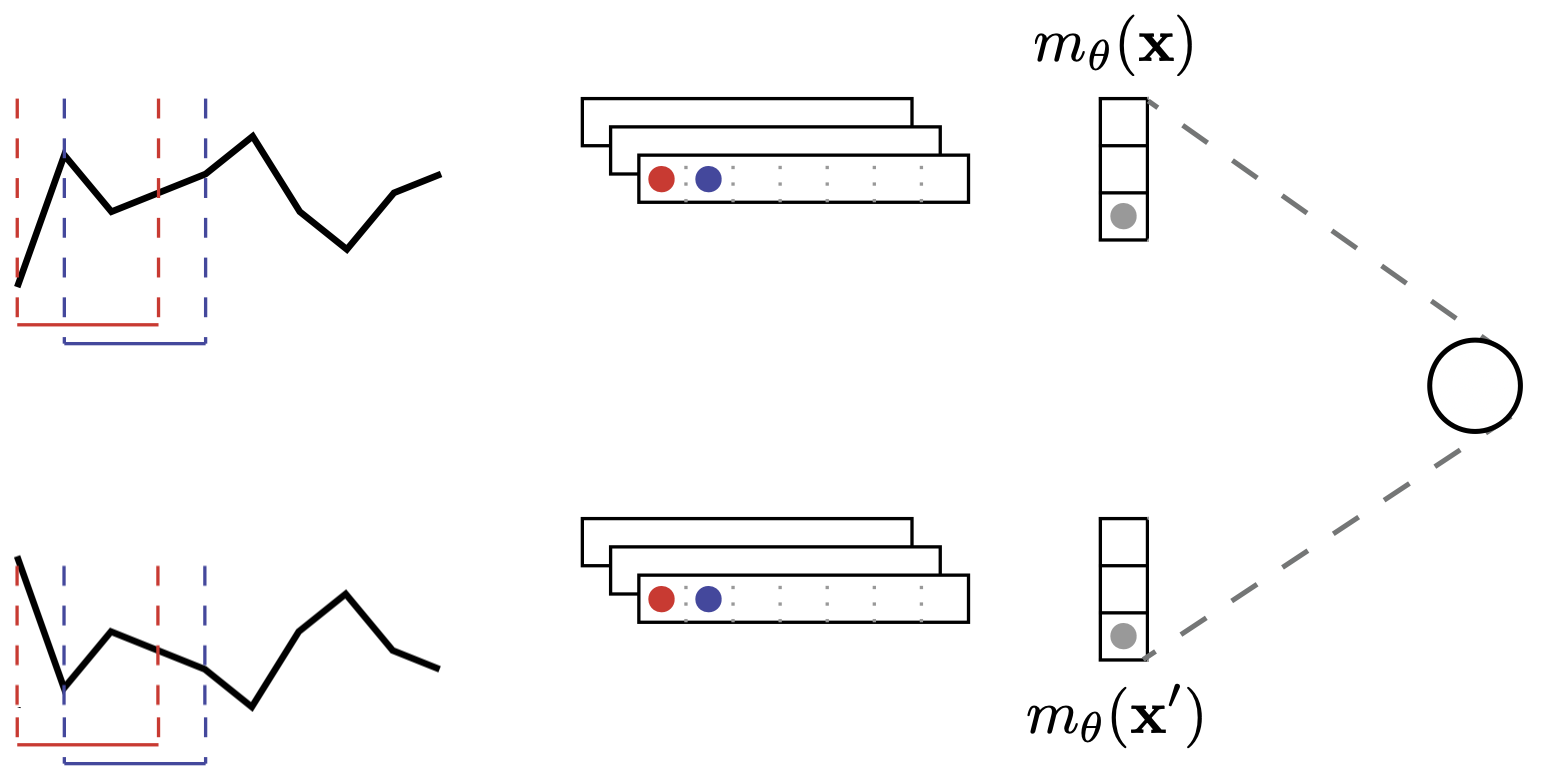
\includegraphics[width=.8\textwidth]{fig/siamese_ldps}
\caption{Shapelet extraction using a Siamese Network. \label{fig:siamese}}
\end{figure}

The resulting model is an instance of a Siamese Network, as illustrated in
Figure~\ref{fig:siamese},
where $m_\theta(\cdot)$ is the feature extraction part of the model that
maps a time series to its shapelet transform representation.
The corresponding loss function on which we optimize is hence

\begin{equation}
    \mathcal{L}(\mathbf{x}, \mathbf{x}^\prime, \beta, \theta) =
        \left(
            DTW(\mathbf{x}, \mathbf{x}^\prime) -
                \beta \| m_\theta(\mathbf{x}) - m_\theta(\mathbf{x}^\prime) \|_2
        \right)^2
\end{equation}

\noindent
where $\beta$ is an additional scale parameter of the model.

We have shown that the resulting model could be used as a feature extractor on top of
which a $k$-means clustering could operate efficiently.
We have also shown in~\cite{carlinisperandio:hal-01841995} that this
representation is useful for time series indexing tasks.%
\footnote{This work is part of Ricardo Carlini Sperandio's PhD thesis.
I am not involved in Ricardo's PhD supervision.}

\subsection{Including Localization Information}

The shapelet transform, as defined above, does not contain localization
information. Several options could be considered to add such
information. First, the global pooling step could be turned into local pooling
to keep track of local shapelet distances.
In~\cite{guilleme:hal-02513295}, we rather focused on augmenting the feature
representation with shapelet match localization features.%
\footnote{This work is part of Mael Guillemé's PhD thesis.
I was not directly involved in Mael's PhD supervision.}

Relying on a set of $p$ random shapelets (shapelets that are extracted
uniformly at
random from the set of all subseries in the training set)
$\{\mathbf{s_k}\}_{k < p}$,
each time series is embedded into a $2p$-dimensional feature that stores, for
each shapelet, the shapelet distance $d_{\mathbf{s_k}}(\cdot)$ as well as
optimal  match localization $l_{\mathbf{s_k}}(\cdot)$:

\begin{eqnarray}
    d_{\mathbf{s_k}}(\mathbf{x}) &=& \min_t
        \|\mathbf{x}_{t \rightarrow t+L_k} - \mathbf{s_k}\|_2 \\
    l_{\mathbf{s_k}}(\mathbf{x}) &=& \arg \min_t
        \|\mathbf{x}_{t \rightarrow t+L_k} - \mathbf{s_k}\|_2
\end{eqnarray}

where $L_k$ is the length of the $k$-th shapelet and
$\mathbf{x}_{t \rightarrow t+L_k}$
is the subseries from $\mathbf{x}$ that starts at timestamp $t$ and has length
$L_k$.

In the random shapelet setting, a large number of shapelets are drawn and
feature selection is used afterwards to focus on most useful shapelets.
In our specific context, we have introduced a structured feature selection
mechanism that allows, for each shapelet, to either:

\begin{itemize}
\item Discard all information (match magnitude and localization),
\item Keep shapelet distance information and discard localization information,
or
\item Keep all information (match magnitude and localization).
\end{itemize}

To do so, we have introduced a modified Sparse-Group-Lasso (called
Semi-Sparse-Group-Lasso) loss that enforces sparsity only on some individual
variables:

\begin{equation}
    \mathcal{L}^{\mathrm{SSGL}}(\mathbf{x}, y, \boldsymbol{\theta}) =
        \mathcal{L}(\mathbf{x}, y, \boldsymbol{\theta})
        + \alpha \lambda
            \left\| \mathbf{M}_\text{ind} \boldsymbol{\beta} \right\|_1
        + (1-\alpha) \lambda \sum_{k=1}^{K} \sqrt{p_k}
            \left\| \boldsymbol{\beta}^{(k)} \right\|_2
\end{equation}

\noindent
where $\mathcal{L}(\cdot,\cdot,\cdot)$ is the unpenalized
loss function,
$\mathbf{M}_\text{ind}$ is a diagonal indicator matrix that has ones on
the diagonal for features that could be discarded individually (localization
features in our random shapelet case), $\boldsymbol{\theta}$ is the set of
all model weights, including weights $\boldsymbol{\beta}$ that are directly
connected to the features (\emph{i.e.}, these are weights from the first layer),
that
are organized in $K$ groups $\boldsymbol{\beta}^{(k)}$ of size $p_k$
($p_k=2$ in the
random shapelet context, each group corresponding to a different shapelet).
Finally, $\alpha$ and $\lambda$ are hyper-parameters of the method that balance
regularizations.

Figure~\ref{fig:ssgl} illustrates the benefit of our SSGL regularization scheme
when groups of variables exist in the data and semi-sparse assumption holds.
One can notice that SSGL slightly outperforms Sparse-Group-Lasso (SGL) in
terms of both Mean Squared Error (MSE) and estimation of zero coefficients.


\begin{figure}[t]
\centering
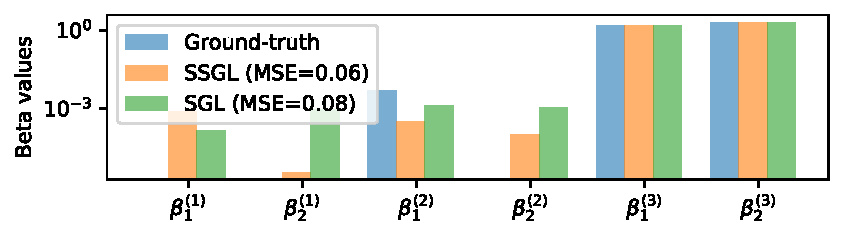
\includegraphics[width=.8\textwidth]{fig/ssgl}
\caption{Semi-Sparse Group Lasso regularization. Coefficients learned using
different regularization schemes for a linear regression problem. Ground-truth
coefficients are reported in blue.
Note that coefficients $\beta_1^{(1)}$, $\beta_2^{(1)}$ and $\beta_2^{(2)}$ are
zero, hence not represented in logscale.
For both SGL and SSGL, the goal is to estimate ground-truth coefficient, hence
the closer their bars are to the blue one (or to 0 when the blue bar is not
visible), the better.
\label{fig:ssgl}}
\end{figure}

When applied to the specific case of random shapelets, we have shown that this
lead to improved accuracy as soon as datasets are large enough for coefficients
to be properly estimated.

\subsection{Learning Shapelets that Look Like Time Series Snippets}

Early works on shapelet-based time series classification relied on a direct
extraction of shapelets as time series snippets from the training set.
Selected shapelets could be used \emph{a posteriori} to explain the classifier's
decision from realistic features.
However, the shapelet enumeration and selection processes were either very
costly or the selection was fast but did not yield good performance.
Jointly learning a shapelet-based representation of the series in the dataset
and classifying the series according to this
representation~\cite{grabocka2014learning} allowed to obtain
discriminative shapelets in a much more efficient way.%
\footnote{This work is part of Yichang Wang's PhD thesis.
I am co-supervising Yichang with Élisa Fromont, Rémi Emonet and Simon
Malinowski.}

However, if the learned shapelets are definitively discriminative, they are
often very different from actual pieces of a real series in the
dataset. As such, these shapelets might not be suited to explain a particular
classifier's decision.
In~\cite{wang2019},
we rely on a simple convolutional network to classify time
series and use an adversarial network that acts as a regularizer to ensure that
learned shapelets are un-distinguishable from actual time series pieces from
the training set.
